\documentclass[frenchb, oneside, headings=normal]{scrartcl}

\usepackage[utf8x]{inputenc}
\usepackage[T1]{fontenc}
\usepackage{lmodern}

\usepackage{ifthen}
\usepackage{url}


\usepackage{multirow}

% Color
% cfr http://en.wikibooks.org/wiki/LaTeX/Colors
\usepackage{color}
\usepackage[usenames,dvipsnames,svgnames,table]{xcolor}
\definecolor{dkgreen}{rgb}{0.25,0.7,0.35}
\definecolor{dkred}{rgb}{0.7,0,0}

\newcommand{\matlab}{\textsc{Matlab}}

% Math symbols
\usepackage{amsmath}
\usepackage{amssymb}
\usepackage{amsthm}
\DeclareMathOperator*{\argmin}{arg\,min}
\DeclareMathOperator*{\argmax}{arg\,max}


% Sets
\newcommand{\Z}{\mathbb{Z}}
\newcommand{\R}{\mathbb{R}}
\newcommand{\Rn}{\R^n}
\newcommand{\Rnn}{\R^{n \times n}}
\newcommand{\C}{\mathbb{C}}
\newcommand{\K}{\mathbb{K}}
\newcommand{\Kn}{\K^n}
\newcommand{\Knn}{\K^{n \times n}}

% Unit vectors
\usepackage{esint}
\usepackage{esvect}
\newcommand{\kmath}{k}
\newcommand{\xunit}{\hat{\imath}}
\newcommand{\yunit}{\hat{\jmath}}
\newcommand{\zunit}{\hat{\kmath}}
\newcommand{\uunit}{\hat{\umath}}

% rot & div & grad & lap
\DeclareMathOperator{\newdiv}{div}
\newcommand{\divn}[1]{\nabla \cdot #1}
\newcommand{\rotn}[1]{\nabla \times #1}
\newcommand{\grad}[1]{\nabla #1}
\newcommand{\gradn}[1]{\nabla #1}
\newcommand{\lap}[1]{\nabla^2 #1}


% Elec
\newcommand{\B}{\vec B}
\newcommand{\E}{\vec E}
\newcommand{\EMF}{\mathcal{E}}
\newcommand{\perm}{\varepsilon} % permittivity

\newcommand{\bigoh}{\mathcal{O}}
\newcommand\eqdef{\triangleq}

\DeclareMathOperator{\newdiff}{d} % use \dif instead
\newcommand{\dif}{\newdiff\!}
\newcommand{\fpart}[2]{\frac{\partial #1}{\partial #2}}
\newcommand{\ffpart}[2]{\frac{\partial^2 #1}{\partial #2^2}}
\newcommand{\fdpart}[3]{\frac{\partial^2 #1}{\partial #2\partial #3}}
\newcommand{\fdif}[2]{\frac{\dif #1}{\dif #2}}
\newcommand{\ffdif}[2]{\frac{\dif^2 #1}{\dif #2^2}}
\newcommand{\constant}{\ensuremath{\mathrm{cst}}}

\usepackage{siunitx}

\usepackage{tikz}

\usepackage{pgfplots}
\usepackage{lmodern}
\usepackage{microtype}
\usepackage{xspace}

\usepackage{babel}
% Listing
% always put it after babel
% http://tex.stackexchange.com/questions/100717/code-in-lstlisting-breaks-document-compile-error
\usepackage{listings}

\definecolor{mygreen}{rgb}{0,0.6,0}
\definecolor{mygray}{rgb}{0.5,0.5,0.5}
\definecolor{mymauve}{rgb}{0.58,0,0.82}
\lstset{ %
  language=Matlab,
  backgroundcolor=\color{white},   % choose the background color; you must add \usepackage{color} or \usepackage{xcolor}
  basicstyle=\footnotesize,        % the size of the fonts that are used for the code
  breakatwhitespace=false,         % sets if automatic breaks should only happen at whitespace
  breaklines=true,                 % sets automatic line breaking
  captionpos=b,                    % sets the caption-position to bottom
  commentstyle=\color{mygreen},    % comment style
  deletekeywords={...},            % if you want to delete keywords from the given language
  escapeinside={\%*}{*)},          % if you want to add LaTeX within your code
  extendedchars=true,              % lets you use non-ASCII characters; for 8-bits encodings only, does not work with UTF-8
  frame=single,	                   % adds a frame around the code
  keepspaces=true,                 % keeps spaces in text, useful for keeping indentation of code (possibly needs columns=flexible)
  keywordstyle=\color{blue},       % keyword style
  otherkeywords={*,...},           % if you want to add more keywords to the set
  numbers=none,                    % where to put the line-numbers; possible values are (none, left, right)
  numbersep=5pt,                   % how far the line-numbers are from the code
  numberstyle=\tiny\color{mygray}, % the style that is used for the line-numbers
  rulecolor=\color{black},         % if not set, the frame-color may be changed on line-breaks within not-black text (e.g. comments (green here))
  showspaces=false,                % show spaces everywhere adding particular underscores; it overrides 'showstringspaces'
  showstringspaces=false,          % underline spaces within strings only
  showtabs=false,                  % show tabs within strings adding particular underscores
  stepnumber=2,                    % the step between two line-numbers. If it's 1, each line will be numbered
  stringstyle=\color{mymauve},     % string literal style
  tabsize=2,	                   % sets default tabsize to 2 spaces
  title=\lstname                   % show the filename of files included with \lstinputlisting; also try caption instead of title
}

\KOMAoptions{DIV=last}

\usepackage[top = 2.5 cm, bottom = 3 cm, left = 2.5 cm, right = 2.5 cm]{geometry}
\usepackage{caption}


\usepackage{epstopdf}
\usepackage{wrapfig}
\begin{document}

\title{Projet ELEC Master 1 - Labo 5}
\subtitle{Groupe 4}
\author{Deprez Damien \and Bilal Ouachalih }
\date{18 november 2016}
\maketitle

The purpose of this lab is to correct the frequency offset and the delay due to the channel.

\section{Questions of the Pre-Lab}

\subsection{Describe what happens to the error rate of your system
when the estimate for the delay in the channel is off by more than one
symbol time}

First, we modified a little bit the scheme os the SlidingCorrelation.vi. In fact, we have added a controller to make an error on the delay and watch what happened. Here is the result

  \begin{minipage}[b]{0.48\linewidth}
        \centering 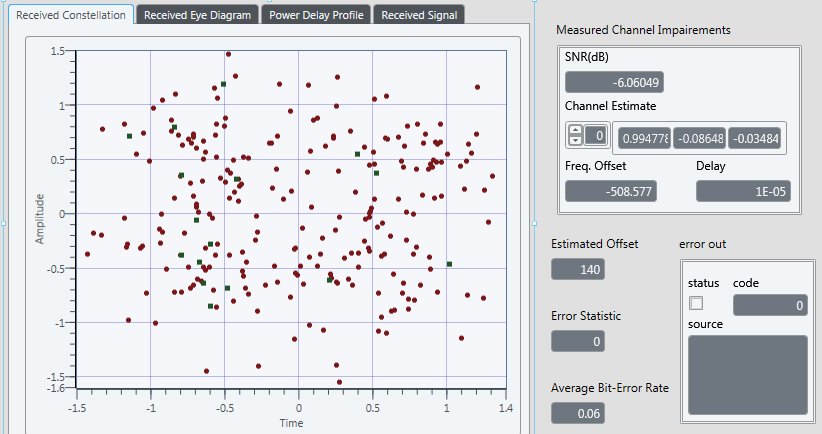
\includegraphics[scale=0.55]{img/Sliding_correletaion_OFF_AWGN_5dB_shift_bit_0}
    %\captionof{figure}{\label{fig1}}
    
    \end{minipage}\hfill
    \begin{minipage}[b]{0.48\linewidth}
         \centering 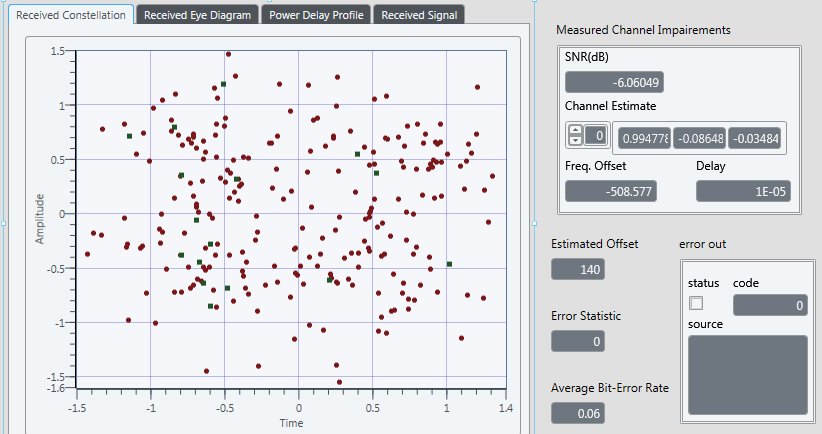
\includegraphics[scale=0.55]{img/Sliding_correletaion_OFF_AWGN_5dB_shift_bit_0}
       % \captionof{figure}{\label{fig2}}
    \end{minipage}
    \begin{minipage}[b]{0.48\linewidth}
        \centering 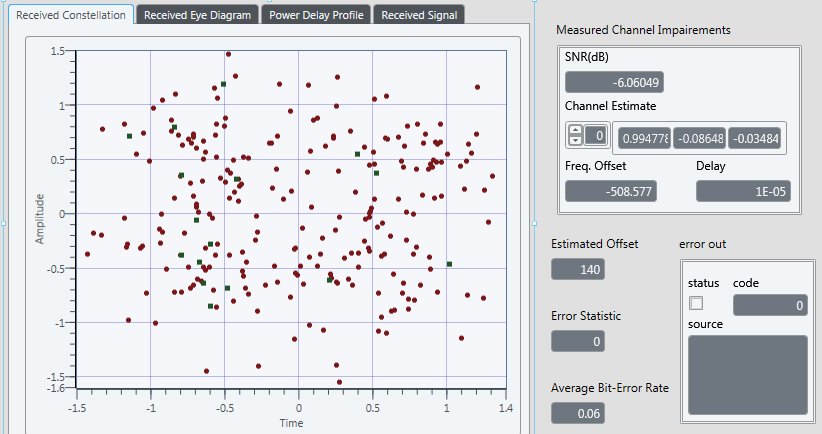
\includegraphics[scale=0.55]{img/Sliding_correletaion_OFF_AWGN_5dB_shift_bit_0.png}
    %\captionof{figure}{\label{fig3}}
    
    \end{minipage}\hfill
    \begin{minipage}[b]{0.48\linewidth}
         \centering 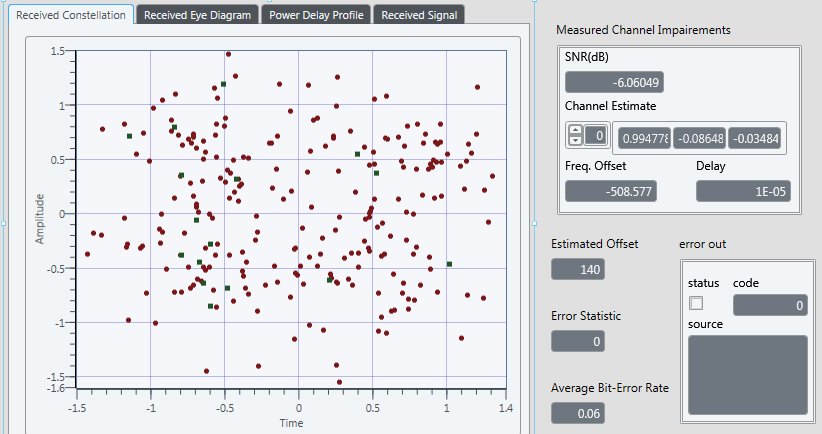
\includegraphics[scale=0.55]{img/Sliding_correletaion_OFF_AWGN_5dB_shift_bit_0.png}
       % \captionof{figure}{\label{fig4}}
    \end{minipage}
    
    \begin{minipage}[b]{0.48\linewidth}
        \centering 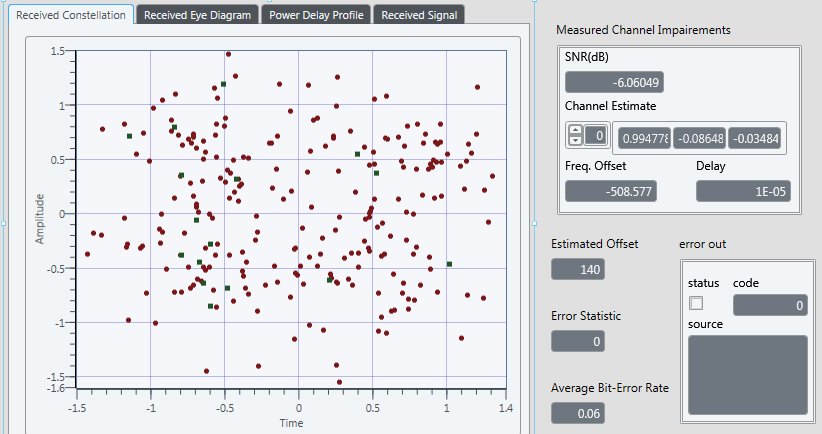
\includegraphics[scale=0.55]{img/Sliding_correletaion_OFF_AWGN_5dB_shift_bit_0.png}
    %\captionof{figure}{\label{fig5}
    
    \end{minipage}\hfill
    \begin{minipage}[b]{0.48\linewidth}
         \centering 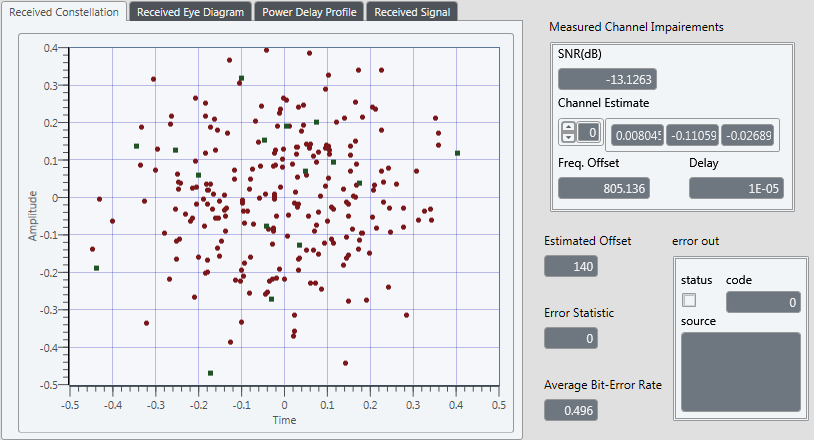
\includegraphics[scale=0.6]{img/Sliding_correletaion_OFF_AWGN_5dB_shift_bit_5.PNG}
        %\captionof{figure}{\label{fig6}}
    \end{minipage}











\end{document}
